\chapter{Тестирование и апробация}

	В этой главе описан процесс тестирования и апробации реализованной системы.

\section{План и методики тестирования}

	Реализованная система адаптивного стриминга видео в нескольких синхронизированных потоках с распределённой сегментированной загрузкой контента должна соответствовать ряду требований, определённых в главе 2, включая как функциональные, так и нефункциональные — в частности, отказоустойчивость и доступность. Проведение сквозного и нагрузочного тестирования является ключевым этапом, обеспечивающим проверку и подтверждение соответствия системы заявленным требованиям.

	Сквозное тестирование (end-to-end) охватывает все этапы работы пользователя с системой — от регистрации и загрузки видео до его последующего воспроизведения в плеере. Оно обеспечивает проверку взаимодействия всех компонентов системы: клиентских интерфейсов, API, сервисов обработки и хранилища данных. Этот вид тестирования будет проводиться в ручном и автоматизированном режиме. Разработка автоматизированных пользовательских сценариев позволит регулярно и быстро проверять основные пользовательские сценарии в текущий момент времени и в будущем. При этом часть компонентов, например, элементы с динамичным интерфейсом, сложно и нецелесообразно покрывать автотестами - для проверки корректности их работы необходимо провести ручное тестирование. Для проведения сквозного тестирования необходимо выполнить следующие шаги:

	\begin{itemize}[label=$\bullet$]
		\item Определить пользовательские сценарии для разных частей системы;
		\item Сформулировать ожидаемые результаты выполнения пользовательских сценариев;
		\item Реализовать автоматизированные сценарии;
		\item Произвести тестирование системы на основе ранее описанных пользовательских сценариев;
		\item Зафиксировать результаты и выявленные отклонения.
	\end{itemize}

	Нагрузочное тестирование дополняет сквозную проверку, позволяя определить отказоустойчивость и доступность системы в условиях пиковых и критических нагрузок. Оно позволяет измерить, с какой нагрузкой система способна справляться без деградации производительности и сбоев. Для проведения нагрузочного тестирования необходимо выполнить следующие шаги:

	\begin{itemize}[label=$\bullet$]
		\item Определить части системы, подверженные наибольшей нагрузке;
		\item Сформулировать метрики оценки производительности и устойчивости системы;
		\item Смоделировать реальные сценарии нагрузки;
		\item Провести тестирование при различных уровнях нагрузки;
		\item Зафиксировать поведение системы и собрать метрики.
	\end{itemize}

	После выполнения сквозного и нагрузочного тестирования будет проведена апробация системы.

\section{Сквозное тестирование}

	Для проверки корректности работы системы определим пользовательские сценарии для видеоплеера и редактора синхронизации, так как они являются точкой входа в приложение для внешних пользователей.

	\begin{itemize}[label=$\bullet$]
		\item Редактор синхронизации:
		\begin{itemize}[label=$\circ$]
			\item Регистрация пользователя: пользователь открывает редактор, вводит логин и пароль, а также повторно пароль в дополнительное поле;
			\item Аутентификация и авторизация пользователя: пользователь открывает редактор, вводит логин и пароль, проходит аутентификацию;
			\item Завершение аутентифицированной сессии: пользователь выходит из аутентифицированной сессии;
			\item Создание нового видео: после аутентификации пользователь создаёт новый экземпляр сущности видео;
			\item Добавление и удаление видеопотоков-кандидатов на загрузку: пользователь добавляет видеопотоки в проект с помощью перетаскивания видео непосредственно в браузер или кнопки загрузки;
			\item Редактирование метаданных видео: пользователь указывает заголовок и описание видео;
			\item Инициация загрузки видеоконтента: пользователь запускает загрузку всех потоков;
			\item Мониторинг прогресса загрузки видеопотоков: пользователь отслеживает прогресс загрузки каждого потока видео в отдельности;
			\item Просмотр результата: после загрузки пользователь переходит на страницу раздачи видео с предварительным отображением видеоплеера, а также возможностью скопировать ссылку для распространения.
		\end{itemize}
		\item Видеоплеер:
		\begin{itemize}[label=$\circ$]
			\item Запуск видеоплеера: пользователь открывает страницу плеера для загруженного ранее видео;
			\item Синхронное воспроизведение: пользователь запускает воспроизведение видео;
			\item Пауза воспроизведения: пользователь останавливает воспроизведение видео;
			\item Перемотка по шкале: пользователь перематывает видео на определённый момент;
			\item Регулировка громкости: пользователь меняет громкость воспроизведения или отключает звук;
			\item Переключение потоков: пользователь переключается между потоками как во время воспроизведения, так и в режиме паузы;
			\item Переключение между режимом воспроизведения: пользователь включает/выключает воспроизведение в полноэкранном режиме.
		\end{itemize}
	\end{itemize}

	Исходя из определённых выше сценариев, для каждого из них сформулированы ожидаемые результаты, которые приведены ниже:

	\begin{itemize}[label=$\bullet$]
		\item Редактор синхронизации:
		\begin{itemize}[label=$\circ$]
			\item Регистрация пользователя: пользователь успешно регистрируется в системе, создаётся новая учётная запись, которая может быть использована для последующей аутентификации;
			\item Аутентификация и авторизация пользователя: введённые учетные данные проверены, при успешной аутентификации пользователь получает доступ к разрешённым разделам интерфейса, при повторном входе в систему спустя длительное время, смена токена аутентификации происходит автоматически, то есть у пользователя нет необходимости входить в систему повторно;
			\item Завершение аутентифицированной сессии: токен аутентификации удаляется, открывается модальное окно авторизации;
			\item Создание нового видео: интерфейс приложения предоставляет возможность создать новый экземпляр видео, отображаются необходимые поля для ввода метаданных, а также форма для управления видеопотоками;
			\item Добавление и удаление видеопотоков-кандидатов на загрузку: пользователь имеет возможность добавлять, удалять потоки видео, управлять их порядком, интерфейс сетки потоков воспроизводит загруженные видео и отображается корректно вне зависимости от порядка действий и не позволяет добавлять более 4 потоков одновременно;
			\item Редактирование метаданных видео: введённые пользователем данные отображаются корректно, при введении большого количества символов в интерфейсе плеера не возникает дефектов;
			\item Инициация загрузки видеоконтента: пользователь не может запустить загрузку при отсутствии введённой информации о метаданных видео;
			\item Мониторинг прогресса загрузки видеопотоков: в интерфейсе в реальном времени отображается прогресс загрузки для каждого потока в отдельности;
			\item Просмотр результата: видеоплеер отображается в интерфейсе корректно, отображается ссылка на видео для интеграции на другие веб-приложения. Кроме того, плеер поддерживает все необходимые интерактивные действия, описанные выше.
		\end{itemize}
		\item Видеоплеер:
		\begin{itemize}[label=$\circ$]
			\item Запуск видеоплеера: интерфейс плеера загружается, все потоки отображаются корректно;
			\item Синхронное воспроизведение: все активные видеопотоки начинают воспроизводиться синхронно
			\item Пауза воспроизведения: все потоки останавливаются одновременно на одной временной позиции
			\item Перемотка по шкале: все потоки синхронно перематываются к указанному времени;
			\item Регулировка громкости: изменения применяются к активному видеопотоку;
			\item Переключение потоков: выбранный поток становится основным, воспроизведение продолжается без рассинхронизации, а также нет явных задержек перед воспроизведением;
			\item Переключение между режимом воспроизведения: видео переключается между режимами воспроизведения, интерфейс масштабируется, воспроизведение продолжается и его качество не меняется.
		\end{itemize}
	\end{itemize}

	Часть пользовательских сценариев, связанных с аутентификацией, авторизацией, а также предварительными действиями перед загрузкой видеоконтента, может быть автоматизирована, поскольку они не зависят от пропускной способности сети и не включают динамический интерфейс, поведение которого может отличаться при разных запусках. Для автоматизации пользовательских сценариев был использован фреймворк Playwright. Он позволяет эмулировать действия реального пользователя в браузере, взаимодействовать DOM-элементами страницы, а также сохранять скриншоты с затемнением динамических элементов. Пример тест кейса, реализованного с помощью Playwright с использованием тестирования на основе скриншотов представлен ниже:

	\begin{lstlisting}[caption={Пример тест-кейса, реализованного с помощью Playwright}]
		test('загрузка видео в потоки', async ({ page }) => {
			const synchronizing = new SynchronizingPage(page);
			
			for (let i = 0; i < UPLOADING_MAX_FLOWS_COUNT; i++) {
				await synchronizing.addFlow();
			}
			
			const flowsGrid = synchronizing.getFlowsGrid();
			
			await expect(flowsGrid).toHaveScreenshot('uploading_grid_init.png');
			
			for (let i = 0; i < UPLOADING_MAX_FLOWS_COUNT; i++) {
				
				await synchronizing.addVideoToFlow(i, videoBuffer);
				
				await expect(flowsGrid).toHaveScreenshot(`uploading_grid_${i + 1}.png`, {
					mask: [
						synchronizing.getVideoLocator(),
					]
				});
			}
		});
	\end{lstlisting}

	Код автоматизированного тестирования представлен в приложении \ref{chap:autotests_code}. Результаты тестирования представлены на рисунке \ref{fig:autotests}.

	\begin{figure}[ht!] 
		\center
		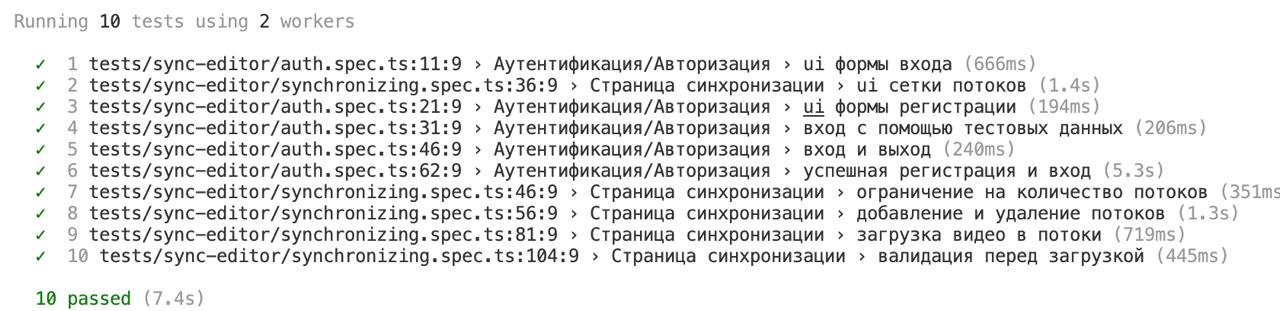
\includegraphics [scale=0.37] {my_folder/images//autotests}
		\caption{Результаты автоматизированного тестирования редактора синхронизации} 
		\label{fig:autotests}  
	\end{figure}

	Пользовательские сценарии, не охваченные автоматизированным тестированием, были проверены с помощью ручного тестирования - результаты приведены в приложении \ref{chap:manual_testing}. По итогам сквозного тестирования ожидаемое поведение системы соответствует фактическому, дефектов не выявлено.

\section{Нагрузочное тестирование}

	После подтверждения корректности выполнения основных пользовательских сценариев в рамках сквозного тестирования можно переходить к нагрузочному тестированию, так как отсутствие критических ошибок в бизнес-логике позволяет сосредоточиться на оценке устойчивости системы. Для этого необходимо определить части системы, которые при работе пользователей испытывают наибольшую нагрузку. Поскольку видеоплеер в основном предоставляет пользователю статический контент, включая видеоданные, файлы js, css, шрифтов и изображений, а основная вычислительная нагрузка при воспроизведении ложится на клиентское устройство, оценка нагрузки на систему со стороны плеера не является репрезентативной для целей нагрузочного тестирования. Редактор синхронизации отправляет гораздо больше запросов к серверу для реализации пользовательских сценариев. Определим распределение запросов к серверу, проанализировав полный жизненный цикл загрузки одного видеопотока объёмом 792 КБ, начиная от авторизации пользователя. Распределение запросов представлено на таблице \ref{tab:distr}.

	\begin{table}[h!]
		\centering
		\begin{tabular}{|l|c|}
			\hline
			\textbf{Запрос к серверу} & \textbf{Количество} \\
			\hline
			\texttt{/upload}         & 100 \\
			\hline
			\texttt{/state}          & 12 \\
			\hline
			\texttt{/me}             & 2 \\
			\hline
			\texttt{/create-video}   & 1 \\
			\hline
		\end{tabular}
		\caption{Частота обращений к серверу по различным эндпоинтам}
		\label{tab:distr}
	\end{table}

	На основе полученной таблицы распределения запросов можно сделать вывод, что наибольшая нагрузка при загрузке видеопотока приходится на эндпоинты upload и state, поэтому при тестирование будет сосредоточено на них.

	Для оценки устойчивости системы к нагрузке в процессе тестирования используются следующие метрики:
	
	\begin{itemize}[label=$\bullet$]
		\item Редактор синхронизации:
		\begin{itemize}[label=$\circ$]
			\item Время отклика HTTP-запроса при пиковой нагрузке, включая:
			\begin{itemize}[label=$\circ$]
				\item avg - среднее значение;
				\item med - медиану;
				\item max - максимальное значение;
				\item p(90) - перцентиль 90%, который характеризует время, за которое завершается 90% всех запросов;
				\item p(95) - перцентиль 95%, который характеризует время, за которое завершается 95% всех запросов.
			\end{itemize}
		\end{itemize}
		\item Доля неуспешных HTTP-запросов;
		\item Общее количество выполненных HTTP-запросов.
	\end{itemize}
	
	Автоматизированный сбор перечисленных выше метрик позволяет проводить инструмент для нагрузочного тестирования K6, который обеспечивает воспроизведение пользовательских сценариев и точную фиксацию показателей.

	Для моделирования реальных сценариев нагрузки необходимо разработать js-скрипт, экспортирующий базовую функцию — пользовательский сценарий, на основе которого будут проводиться измерения производительности системы.

	Однако для моделирования сценария загрузки и периодического опрашивания состояния видео предварительно необходимо провести аутентификацию пользователя, чтобы была возможность загружать видео сегменты. Функция setup в K6 предназначена для выполнения подготовительных действий перед началом нагрузочного теста, поэтому процесс аутентификации необходимо реализовать в ней.
	
	Для поддержания гибкости тестирования системы в разных окружениях данные для аутентификации, а также адрес API-Шлюза были вынесены в переменные окружения USER\_EMAIL, USER\_PASSWORD и BASE\_GATEWAY\_URL. Данные, которые возвращаются в результате выполнения setup передаются на вход основной функции для тестирования.

	Основная функция для тестирования принимает в качестве аргумента accessToken и использует его для создания видео, а также загрузки бинарных данных его потоков. Эта функция выполняется отдельно для каждого виртуального пользователя. Виртуальные пользователи используются для эмуляции одновременной работы множества реальных пользователей с системой. Код сценария представлен в приложении \ref{chap:load_testing_code}.

	Для оценки реакции системы на возрастающую нагрузку, а также для анализа тренда изменения времени отклика, необходимо провести серию тестов при различном количестве одновременно работающих виртуальных пользователей.

	Результаты тестирования с использованием ранее описанных метрик при различных уровнях нагрузки, моделируемых разным количеством виртуальных пользователей, представлены в таблице \ref{tab:load_testing_results}. Тестирование проводилось при развертывании системы на устройстве с процессором Apple Silicon M1, 8‑Core CPU и 16 ГБ оперативной памяти. Все компоненты системы, включая клиентскую часть, сервер API и сервисы обработки, были развернуты и запущены на одном физическом устройстве.

	\begin{table}[h!]
		\centering
		\renewcommand{\arraystretch}{1.2}
		\begin{tabular}{|p{1.5cm}|c|c|c|c|c|c|p{2cm}|}
			\hline
			\textbf{VU} & \textbf{avg, мс} & \textbf{min, мс} & \textbf{med, мс} & \textbf{max, мс} & \textbf{p(90), мс} & \textbf{p(95), мс} & \textbf{Запросы} \\
			\hline
			5   & 13.06 & 1.54 & 7.43  & 172.75 & 24.23  & 40.97  & 116 \\
			\hline
			20  & 37.76 & 1.87 & 15.6  & 667.06 & 73.64  & 124.02 & 461 \\
			\hline
			40  & 71.78 & 1.98 & 35.3  & 1210.0 & 128.04 & 215.87 & 911 \\
			\hline
			80  & 159.09 & 2.17 & 81.37  & 2580.0 & 319.75 & 524.96 & 1835 \\
			\hline
			100 & 179.8  & 1.85 & 109.14 & 2570.0 & 357.71 & 592.48 & 2257 \\
			\hline
			125 & 249.17 & 1.9  & 132.94 & 3930.0 & 513.89 & 900.02 & 2850 \\
			\hline
		\end{tabular}
		\caption{Результаты нагрузочного тестирования}
		\label{tab:load_testing_results}
	\end{table}

	В таблице не указана доля неуспешных запросов, так как в ходе проведения тестирования этот показатель составлял 0\% при любом количестве виртуальных пользователей. Для наглядной интерпретации полученных результатов проведено графическое представление зависимости времени отклика от количества виртуальных пользователей. График зависимости представлен на рисунке \ref{fig:load_testing_graphic}.

	\begin{figure}[ht!] 
		\center
		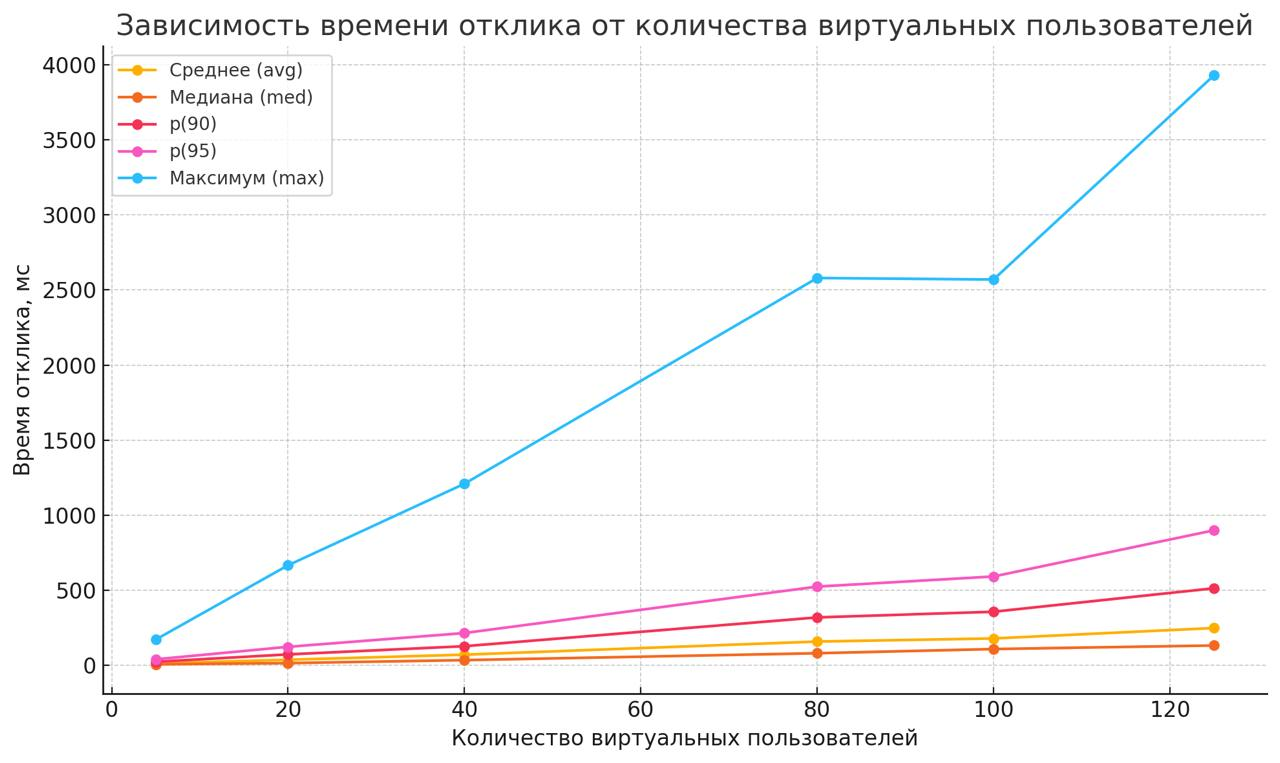
\includegraphics [scale=0.37] {my_folder/images//load_testing_graphic}
		\caption{График зависимости времени отклика от количества виртуальных пользователей} 
		\label{fig:load_testing_graphic}  
	\end{figure}

	На графике видно, что увеличение времени отклика происходит пропорционально росту количества одновременно работающих виртуальных пользователей. Это говорит о сохранении отказоустойчивости и доступности системы: при возрастании нагрузки не наблюдается резкого ухудшения отклика, а поведение системы остаётся предсказуемым и контролируемым, без перехода в критические режимы деградации.

	Кроме того, на основе полученных в ходе тестирования метрик можно определить значение количества запросов в секунду ($RPS$), которое система способна обрабатывать при пиковой нагрузке. Расчёт производится по формуле, представленной ниже, где $\overline{t}_{\text{resp}}$ — среднее время отклика системы на один запрос, а $N$ — количество виртуальных пользователей.

	\[
	\text{RPS} = \frac{1}{\overline{t}_{\text{resp}}} \times N
	\]

	Подставив в указанную формулу экспериментальные данные, зафиксированные при пиковой нагрузке в 125 одновременно активных пользователей, получаем значение порядка 501 запроса в секунду. Рассчёты представлены ниже.
	
	\[
	\text{RPS} = \frac{1}{0{,}24917} \times 125 \approx 501{,}67
	\]

	Это свидетельствует о высоком уровне доступности и устойчивости системы при пиковых значениях нагрузки.

	\section{Апробация}

	Разработанная в предыдущих главах система, включающая редактор синхронизации и встроенный видеоплеер, была размещена на хостинговой платформе и протестирована реальными пользователями. Доступ к системе был предоставлен ограниченной группе участников с целью анализа удобства и эффективности взаимодействия с системой.

	По завершении работы с системой пользователи заполнили анкету, в которой по десятибалльной шкале оценили ряд параметров, отражающих удобство, стабильность и функциональность системы, представленных ниже:

	\begin{itemize}[label=$\bullet$]
		\item Удобство и интуитивность интерфейса редактора синхронизации;
		\item Точность и отзывчивость синхронизации медиа-контента;
		\item Удобство навигации и управления воспроизведением;
		\item Качество и стабильность работы встроенного видеоплеера;
		\item Общая производительность и стабильность системы при работе с медиафайлами;
		\item Вероятность использования системы для размещения синхронизированного мультимедийного контента на собственной платформе.
	\end{itemize}

	В анкетировании приняли участие 42 человека, усреднённые оценки которых приведены в таблице \ref{tab:survey_results}.

	\begin{table}[h!]
		\centering
		\renewcommand{\arraystretch}{1.3}
		\begin{tabular}{|p{9cm}|c|}
			\hline
			\textbf{Оцениваемый параметр} & \textbf{Средняя оценка} \\
			\hline
			Удобство и интуитивность интерфейса редактора синхронизации & 8.90 \\
			\hline
			Точность и отзывчивость синхронизации медиа-контента & 8.43 \\
			\hline
			Качество и стабильность работы встроенного видеоплеера & 8.86 \\
			\hline
			Удобство навигации и управления воспроизведением & 9.00 \\
			\hline
			Общая производительность и стабильность системы при работе с медиафайлами & 8.36 \\
			\hline
			Вероятность использования системы для размещения синхронизированного мультимедийного контента на собственной платформе & 9.43 \\
			\hline
		\end{tabular}
		\caption{Усреднённые оценки параметров системы по результатам анкетирования}
		\label{tab:survey_results}
	\end{table}

	Анкетирование показало, что система удобна в использовании, стабильно работает и может эффективно применяться для размещения и воспроизведения синхронизированного мультимедийного контента на собственной платформе.

	\section{Выводы}

	В этой главе было проведено сквозное, нагрузочное тестирование и апробация системы. Результаты показали, что система стабильно функционирует при различных сценариях использования и выдерживает высокую нагрузку без сбоев. Отзывы пользователей подтвердили удобство и надёжность интерфейса. Таким образом, система соответствует заявленным функциональным и нефункциональным требованиям.